 

%%%%%%%%%%%%%%%%%%%%%%%%%%%%%%%%%%%%%%%%%%OBJETIVOS 

%%%%%%%%%%%%%%%%%%%%%%%%%%%%%%%%%%%%%%%%%%EQUIPOS Y MATERIALES 

%%%%%%%%%%%%%%%%%%%%%%%%%%%%%%%%%%%%%%%%%%INTRODUCCIÓN 
   
%%%%%%%%%%%%%%%%%%%%%%%%%%%%%%%%%%%%%%%%%%CONCLUSIONES 

\documentclass[a4paper,12pt]{article} % Tipo de documento

% Paquetes
\usepackage[utf8]{inputenc} % Codificación de caracteres
\usepackage[spanish]{babel}  % Idioma español
\usepackage{amsmath}         % Paquete para matemáticas
\usepackage{graphicx}        % Para incluir imágenes
\usepackage{hyperref}        % Para enlaces

\title{Taller 1 Maquinas Electricas} % Título del documento
\author{Daniel Fernando Aranda Contreras} % Autor del documento
\date{\today} % Fecha actual, puedes cambiarla por una fecha específica

\begin{document}

\maketitle % Genera el título

\begin{abstract}
    
    Este es un resumen de tu documento. Aquí puedes describir brevemente el contenido y los objetivos del mismo.
\end{abstract}

\section{OBJETIVOS }
Aquí comienza la introducción de tu documento. Explica el tema y la motivación detrás de tu trabajo.
    
\section{EQUIPOS Y MATERIALES}
\begin{figure}[h] % 'h' indica que la imagen se coloca aquí
    \centering
    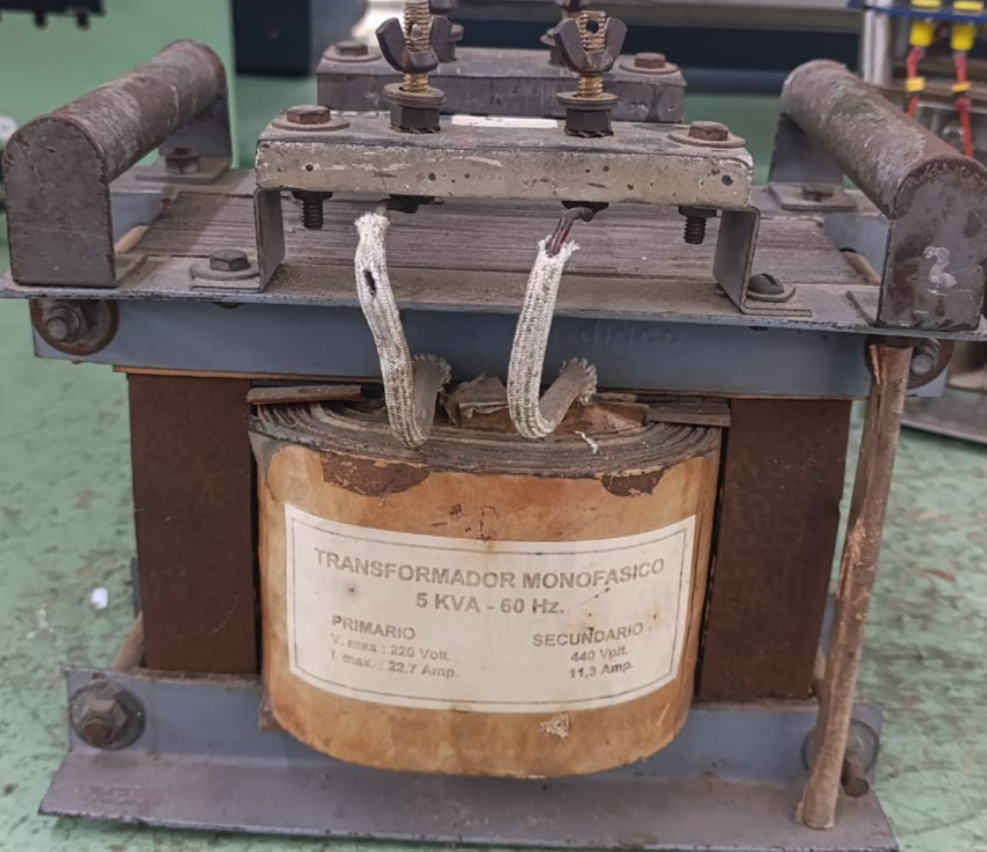
\includegraphics[width=0.5\textwidth]{img/Transformador monofasico.png} % Cambia la ruta a tu imagen
    \caption{Ficha tecnica del transformador monofasico.}
    \label{fig:mi_imagen}
\end{figure}

\begin{figure}[h] % 'h' indica que la imagen se coloca aquí
    \centering
    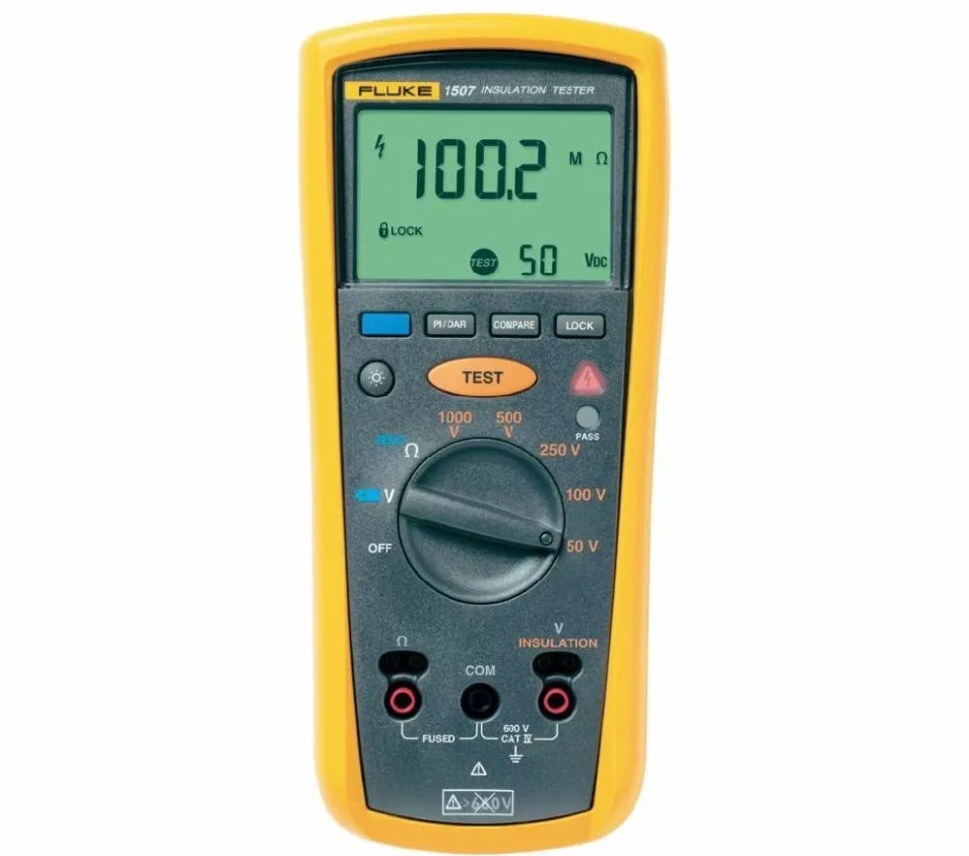
\includegraphics[width=0.5\textwidth]{img/Megahometro megger.png} % Cambia la ruta a tu imagen
    \caption{Megahometro Fluke 1507.}
    \label{fig:megahometro}
\end{figure}

\begin{figure}[h] % 'h' indica que la imagen se coloca aquí
    \centering
    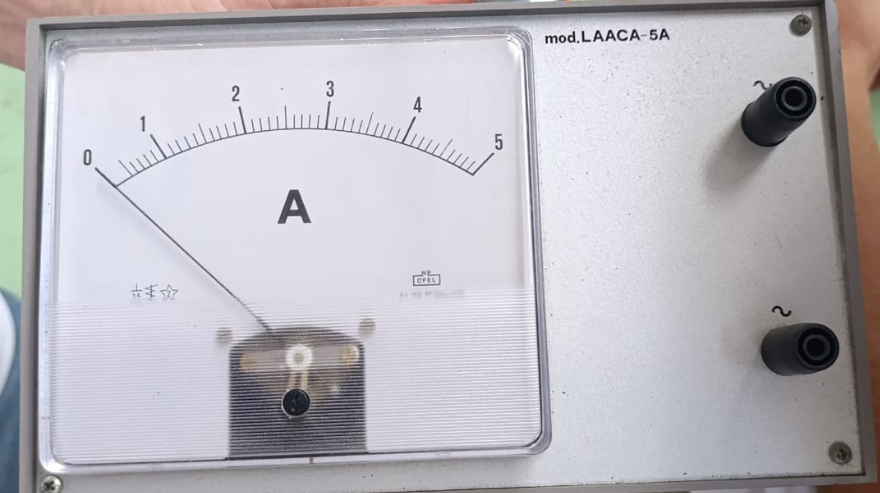
\includegraphics[width=0.5\textwidth]{img/Amperimetro Analogico.png} % Cambia la ruta a tu imagen
    \caption{Amperimetro Analogico.}
    \label{fig:AmpAnalogico}
\end{figure}



\begin{figure}[h] % 'h' indica que la imagen se coloca aquí
    \centering
    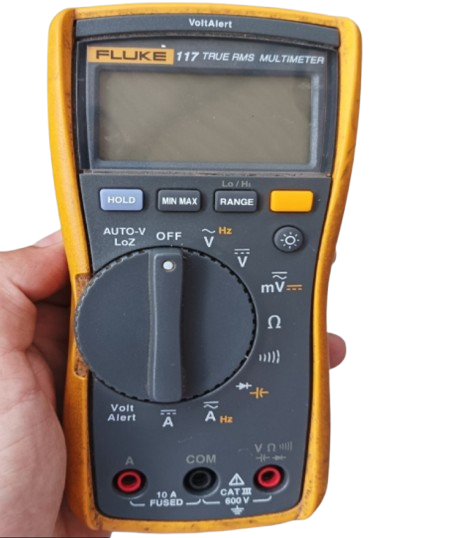
\includegraphics[width=0.5\textwidth]{img/Multimetro digital.png} % Cambia la ruta a tu imagen
    \caption{Multimetro Fluke 117.}
    \label{fig:MulDigital}
\end{figure}





\subsection{Subsección 2}
Desarrollo de la segunda subsección.

\section{INTRODUCCIÓN }
Aquí puedes presentar los resultados que has obtenido. Puedes usar tablas y gráficos si es necesario.

\section{CONCLUSIONES}
En esta sección se presentan las conclusiones de tu trabajo.

\begin{thebibliography}{99}
% Aquí puedes incluir tus referencias
\bibitem{ref1} Autor. Título del libro. Editorial, Año.
\bibitem{ref2} Autor. Título del artículo. Revista, Año.
\end{thebibliography}

\end{document}
